\cleardoublepage
\chapter{PENDAHULUAN}
\label{chap:pendahuluan}


\section{Latar Belakang}
\label{sec:bab1-latar-belakang}

Diabetes melitus tipe 1 (DMT1) merupakan penyakit kronis yang ditandai oleh kerusakan sel beta pankreas sehingga tubuh mengalami defisiensi insulin dan memerlukan terapi 
insulin eksogen secara berkelanjutan \parencite{ada2026}. Karena itu, pengelolaan DMT1 tidak berhenti pada pemberian insulin, tetapi menuntut penyesuaian terus-menerus
terhadap perubahan kadar glukosa dan berbagai faktor yang memengaruhinya. Dalam konteks Indonesia, pengelolaan DMT1 juga menghadapi tantangan berupa keterlambatan diagnosis dan keterbatasan 
pendampingan oleh tenaga kesehatan dengan kompetensi yang sesuai, terutama pada populasi anak \parencite{pulungan2021,faizi2025}. 

Pengelolaan tersebut semakin penting karena risiko kadar glukosa yang terlalu tinggi dan terlalu rendah tidak setara. Kadar yang terlalu tinggi menimbulkan kerusakan dalam
jangka panjang, sedangkan kadar yang terlalu rendah menimbulkan konsekuensi akut. Pengendalian glikemik yang lebih ketat terbukti menurunkan risiko komplikasi mikrovaskular,
tetapi intensifikasi terapi juga meningkatkan risiko hipoglikemia \parencite{nathan2014}. Oleh sebab itu, pengelolaan DMT1 tidak cukup hanya menurunkan kadar glukosa; kadar
tersebut harus dipertahankan dalam rentang yang aman, dan perubahan yang dapat terjadi dalam waktu singkat perlu diantisipasi. 

Antisipasi tersebut tidak sederhana karena kadar glukosa dipengaruhi oleh berbagai faktor yang bekerja pada skala waktu berbeda. Asupan karbohidrat memengaruhi kadar
glukosa melalui penyerapan makanan dan respons insulin \parencite{bergman1979,dallaman2014}. Aktivitas fisik memengaruhi penggunaan glukosa dan sensitivitas insulin
\parencite{colberg2016}, dan stres psikologis dapat memengaruhi kadar serta variabilitas glukosa \parencite{velasco2022}. Akibatnya, keadaan glukosa pada suatu waktu tidak
dapat dipahami secara memadai dari satu nilai pengukuran saja. Riwayat pengukuran dan kejadian sebelumnya diperlukan untuk memperkirakan arah perubahan yang sedang
berlangsung dan untuk membedakan perubahan bertahap dari perubahan yang cepat. Semakin jarang pengukuran dilakukan, semakin penting riwayat tersebut untuk memperkirakan
kondisi glukosa berikutnya.

Kebutuhan akan informasi tersebut berhadapan dengan ketidakmerataan akses terhadap teknologi pemantauan. \textit{Continuous glucose monitoring} (CGM) menghasilkan deret
pengukuran yang rapat sehingga perubahan kadar glukosa dapat diamati secara rinci. Namun, akses terhadap teknologi diabetes masih dibatasi oleh biaya dan ketersediaan
perangkat, terutama di negara berkembang \parencite{santoscastro2025}. Di Indonesia, penggunaan glukometer dan strip pengukuran juga memberikan beban biaya berulang bagi sebagian 
pasien \parencite{ramadaniati2024}. Kondisi tersebut membuat pilihan pemantauan tidak selalu ditentukan oleh kebutuhan klinis saja, tetapi juga oleh keterjangkauan perangkat 
dan sumber daya yang tersedia.

Dalam kondisi tersebut, pemantauan \textit{finger-stick} yang dicatat secara periodik menjadi sumber data yang lebih sesuai dengan keadaan sasaran. Karakteristiknya
berbeda dari CGM: pengukuran tidak berlangsung kontinu dan jarak antarpembacaan bervariasi, sehingga ada rentang waktu ketika keadaan glukosa tidak teramati sama sekali.
Dataset OhioT1DM memuat kanal CGM dan \textit{finger-stick} sekaligus, dengan karakteristik pengamatan yang berbeda \parencite{marling2020}. Karena rentang yang tidak
teramati itu, kemampuan memperkirakan keadaan setelah pengukuran terakhir menjadi semakin penting ketika pemantauan semakin jarang.

Pendekatan pembelajaran berbasis data telah digunakan untuk memperkirakan dinamika kadar glukosa dari riwayat pengukuran dan variabel pendukung \parencite{woldaregay2019}. 
Prediksi tersebut dapat menyediakan informasi mengenai keadaan glukosa yang mungkin terjadi pada waktu berikutnya. Namun, keluaran berupa angka prediksi belum secara otomatis 
menjawab kebutuhan berikutnya dalam pengambilan keputusan klinis, yaitu bagaimana menginterpretasikan keadaan tersebut dan pengetahuan klinis apa yang relevan untuk ditinjau.

Kebutuhan tersebut berkaitan dengan peran \textit{clinical decision support system} (CDSS). CDSS menyediakan informasi yang mendukung pengambilan keputusan klinis dan pada
prinsipnya tidak menggantikan penilaian tenaga kesehatan \parencite{sutton2020}. Karena itu, dalam pengelolaan DMT1, informasi prediksi akan lebih berguna apabila
dihubungkan dengan pengetahuan klinis yang relevan dan tetap dapat diperiksa oleh dokter, bukan berhenti sebagai angka yang harus ditafsirkan sendiri.

Salah satu pendekatan yang dapat digunakan untuk menghubungkan model bahasa dengan sumber pengetahuan adalah \textit{Retrieval-Augmented Generation} (RAG). RAG menggabungkan
penelusuran dokumen eksternal dengan proses \textit{generation} sehingga jawaban bersandar pada dokumen yang dijadikan konteks \parencite{lewis2020,gao2023}. 
Pendekatan tersebut telah diterapkan pada penafsiran pedoman klinis. \textcite{kresevic2024} mengembangkan pendekatan RAG untuk membantu penafsiran pedoman klinis dalam sistem pendukung 
keputusan dan melaporkan peningkatan akurasi dibandingkan model tanpa penelusuran. Penelitian lain juga menerapkan RAG pada domain diabetes untuk 
kebutuhan edukasi dan tanya jawab berbasis dokumen \parencite{lee2024,wang2024}.

Meskipun demikian, masih ada persoalan mengenai kondisi apa yang dijadikan dasar penelusuran. Penelitian RAG klinis yang ditelaah menyusun penelusuran dari pertanyaan
atau dari kondisi pasien saat ini yang diberikan kepada sistem \parencite{kresevic2024,lee2024,wang2024}. Penelitian \textit{Active RAG} oleh \textcite{jiang2023} memperkenalkan 
penelusuran yang bersifat antisipatif, tetapi kondisi pemicunya berasal dari prediksi model bahasa terhadap teks yang sedang dihasilkan, bukan dari prediksi eksternal mengenai 
keadaan fisiologis pasien. Pada sisi lain, penelitian berbasis \textit{personal health knowledge graph} memperlihatkan kemungkinan mengintegrasikan data 
kesehatan personal, prediksi, dan rekomendasi, tetapi pendekatan tersebut membutuhkan integrasi data dan representasi pengetahuan yang lebih kompleks \parencite{rad2024}.

Keterbatasan infrastruktur juga tidak hanya berkaitan dengan perangkat pemantauan. Pada layanan primer di Indonesia, keterbatasan pengetahuan penyedia layanan mengenai tata 
laksana diabetes dan alur rujukan masih ditemukan, sementara pencapaian pengendalian diabetes di tingkat nasional juga masih menjadi tantangan \parencite{hustrini2026,muharram2025}. 
Kajian pada negara berpendapatan rendah menunjukkan persoalan serupa berupa keterbatasan insulin dan logistik, kesinambungan perawatan, serta keterbatasan kapasitas sistem 
layanan \parencite{owusu2024}. Kondisi tersebut menunjukkan bahwa solusi digital untuk pengelolaan DMT1 perlu mempertimbangkan keterbatasan infrastruktur dan kesinambungan 
pengambilan keputusan, selain menghasilkan informasi yang relevan secara klinis.

Dalam konteks tersebut, pendekatan yang menghubungkan prediksi dengan pengetahuan klinis perlu mempertahankan fungsi antisipatif tanpa bergantung pada integrasi infrastruktur 
yang berat. Kajian mengenai teknologi diabetes menunjukkan bahwa kemampuan pemantauan dan pengelolaan terus meluas, tetapi penerapannya pada lingkungan dengan sumber daya
terbatas tetap dibatasi oleh ketersediaan perangkat, biaya, dan kesiapan sistem layanan \parencite{samajdar2025}. Karena itu, diperlukan alur 
pendukung keputusan yang memanfaatkan informasi yang tersedia, menggunakan prediksi sebagai dasar antisipasi, serta tetap menempatkan tenaga kesehatan sebagai pihak yang 
melakukan penilaian akhir.

Dari rangkaian penelitian tersebut terlihat adanya ruang integrasi antara prediksi kondisi glukosa dan penelusuran pengetahuan klinis. Salah satu peluangnya adalah menyusun
kueri penelusuran pedoman dari kondisi fisiologis yang diprediksi, sebelum kondisi tersebut benar-benar terjadi. Pendekatan ini relevan pada lingkungan dengan pemantauan
yang tidak kontinu karena prediksi memberi waktu untuk menyiapkan informasi klinis yang sesuai. Atas dasar itu, penelitian ini membangun artefak yang menghubungkan
prediksi kadar glukosa dengan penelusuran pedoman klinis melalui \textit{query transformation} terkondisi-prediksi, lalu mengintegrasikannya ke dalam CDSS beralur
\textit{doctor-mediated}. Celah penelitian (\textit{research gap}) yang diisi adalah belum adanya alur pendukung keputusan yang menghubungkan prediksi kondisi fisiologis
mendatang, penelusuran pedoman klinis, dan penyusunan rekomendasi pada lingkungan dengan keterbatasan infrastruktur.

\section{Rumusan Masalah}
\label{sec:bab1-rumusan-masalah}

Berdasarkan latar belakang tersebut, yaitu keterbatasan pemantauan, kebutuhan akan prediksi, dan peluang integrasi antara prediksi fisiologis dan penelusuran pengetahuan
klinis, penelitian ini merumuskan tiga pertanyaan penelitian sebagai berikut.

\begin{enumerate}
    \item Bagaimana merancang dan mengimplementasikan modul prediksi kadar glukosa DMT1 yang dapat mengolah data dengan karakteristik pemantauan berbeda dan dapat berjalan
    pada lingkungan komputasi terbatas?
    \item Bagaimana merancang dan mengimplementasikan \textit{query transformation} terkondisi-prediksi agar penelusuran pedoman klinis menggunakan keadaan glukosa yang 
    diprediksi?
    \item Bagaimana mengintegrasikan modul prediksi dan mekanisme RAG terkondisi-prediksi menjadi CDSS \textit{doctor-mediated} yang sesuai dengan keterbatasan infrastruktur?
\end{enumerate}

\section{Tujuan Penelitian}
\label{sec:bab1-tujuan}

Sejalan dengan rumusan masalah tersebut, penelitian ini memiliki tiga tujuan sebagai berikut.

\begin{enumerate}
    \item Merancang dan mengimplementasikan modul prediksi kadar glukosa penyandang DMT1 berbasis pembelajaran mesin yang dapat memanfaatkan data pemantauan dengan 
    karakteristik kerapatan berbeda serta berjalan pada lingkungan komputasi terbatas.
    \item Merancang dan mengimplementasikan mekanisme \textit{Retrieval-Augmented Generation} dengan \textit{query transformation} terkondisi-prediksi yang menggunakan keadaan 
    glukosa terprediksi sebagai dasar penelusuran pedoman klinis.
    \item Mengintegrasikan modul prediksi dan mekanisme RAG terkondisi-prediksi ke dalam sistem pendukung keputusan klinis beralur \textit{doctor-mediated} yang dapat digunakan
    pada lingkungan dengan keterbatasan infrastruktur.
\end{enumerate}

\section{Batasan Masalah}
\label{sec:bab1-batasan}

Untuk menjaga penelitian tetap berada dalam ruang lingkup tugas akhir, batasan masalah yang digunakan adalah sebagai berikut.

\begin{enumerate}
    \item \textbf{Ruang lingkup penyakit.} Penelitian difokuskan pada diabetes melitus tipe 1 (DMT1). Tipe diabetes lain berada di luar cakupan penelitian.

    \item \textbf{Sumber data.} Penelitian menggunakan dataset publik OhioT1DM sebagai sumber data utama. Skenario pemantauan mandiri menggunakan kanal finger-stick 
    yang benar-benar tersedia pada dataset dan bukan hasil penjarangan buatan dari kanal CGM \parencite{marling2020}.

    \item \textbf{Representasi pasien.} Pada skenario aplikasi sasaran, keadaan pasien direpresentasikan dari catatan \textit{logbook}, bukan dari aliran sensor kontinu; kanal CGM
    pada dataset digunakan untuk melatih dan mengevaluasi model, bukan sebagai masukan langsung aplikasi.

    \item \textbf{Horizon prediksi.} Kanal CGM dibatasi pada horizon +30 menit dan +60 menit. Skenario \textit{finger-stick} menggunakan horizon sekitar 240 menit sesuai konfigurasi produksi final
    yang ditetapkan pada artefak implementasi.

    \item \textbf{Peran sistem.} Sistem dibatasi sebagai \textit{clinical decision support system} dengan alur \textit{doctor-mediated}. Rekomendasi menjadi bahan pertimbangan
     yang harus ditinjau oleh dokter dan sistem tidak dimaksudkan untuk mengambil keputusan klinis secara otonom \parencite{sutton2020}.

    \item \textbf{Lingkungan komputasi.} Komputasi inti ditujukan untuk berjalan pada perangkat kelas konsumen tanpa akselerator grafis khusus. Tahap pembangkitan bahasa alami 
    dapat menggunakan layanan berbasis awan sehingga ketersediaan konektivitas menjadi salah satu batasan operasional.

    \item \textbf{Basis pengetahuan.} Penelusuran dibatasi pada korpus pedoman klinis yang dikurasi; dokumen dipilih agar mencakup kondisi glukosa dan variabel yang
    dapat dikenali sistem dari data penelitian.

    \item \textbf{Sifat penelitian.} Penelitian bersifat \textit{proof-of-concept} dan tidak mencakup uji klinis terkontrol pada pasien nyata.

    \item \textbf{Validitas eksternal.} Generalisasi hasil dibatasi oleh karakteristik dataset OhioT1DM, termasuk jumlah pasien, karakteristik populasi, dan perbedaan konteks 
    terapi antara dataset dengan konteks penerapan sasaran.

    \item \textbf{Faktor musiman dan keagamaan.} Pengaruh musim dan hari besar keagamaan tidak dianalisis karena dokumentasi OhioT1DM menyatakan bahwa proses de-identifikasi 
    temporal menggeser bulan pada catatan waktu sehingga analisis musim tidak dapat dilakukan secara valid \parencite{marling2020}.
\end{enumerate}

\section{Metodologi Penelitian}
\label{sec:bab1-metodologi}

Penelitian ini menggunakan \textit{Design Science Research Methodology} (DSRM) sebagai kerangka metodologis utama. DSRM menempatkan pembangunan artefak sebagai pusat kegiatan 
penelitian melalui tahapan identifikasi masalah dan motivasi, definisi tujuan solusi, desain dan pengembangan, demonstrasi, evaluasi, dan komunikasi \parencite{peffers2007}.

Sebagai pembanding, \textit{Design Research Methodology} (DRM) juga dipertimbangkan. DRM menempatkan proses perancangan sebagai objek penelitian, sedangkan penelitian ini 
berorientasi pada pembangunan artefak perangkat lunak untuk menjawab masalah yang telah diidentifikasi, sehingga fokus kedua kerangka tersebut berbeda \parencite{blessing2009}. 
Berdasarkan perbedaan objek tersebut, DSRM dipilih sebagai kerangka yang sesuai.

Pemetaan aktivitas DSRM terhadap laporan ini adalah sebagai berikut.

\begin{enumerate}
    \item \textbf{Identifikasi masalah dan motivasi} direalisasikan melalui Bab I dan didukung oleh kajian literatur pada Bab II.
    \item \textbf{Definisi tujuan solusi} direalisasikan melalui analisis masalah, kebutuhan, data, dan alternatif solusi pada Bab III.
    \item \textbf{Perancangan dan pengembangan} direalisasikan melalui perancangan dan pembangunan artefak pada Bab IV dan Bab V.
    \item \textbf{Demonstrasi} direalisasikan melalui penggunaan artefak pada skenario yang merepresentasikan alur konsultasi berbasis data logbook pada Bab V.
    \item \textbf{Evaluasi} direalisasikan pada Bab VI untuk memperoleh bukti terhadap pemenuhan kebutuhan dan tujuan penelitian.
    \item \textbf{Komunikasi} direalisasikan melalui penyajian hasil, kontribusi, keterbatasan, dan saran pengembangan pada Bab VII.
\end{enumerate}

Pemetaan aktivitas tersebut terhadap struktur laporan ditunjukkan pada Gambar~\ref{fig:fig1.1_dsrm}. Pemetaan ini menjaga keterkaitan antara tahapan penelitian dan
struktur laporan.

\begin{figure}[!htbp]
    \centering
    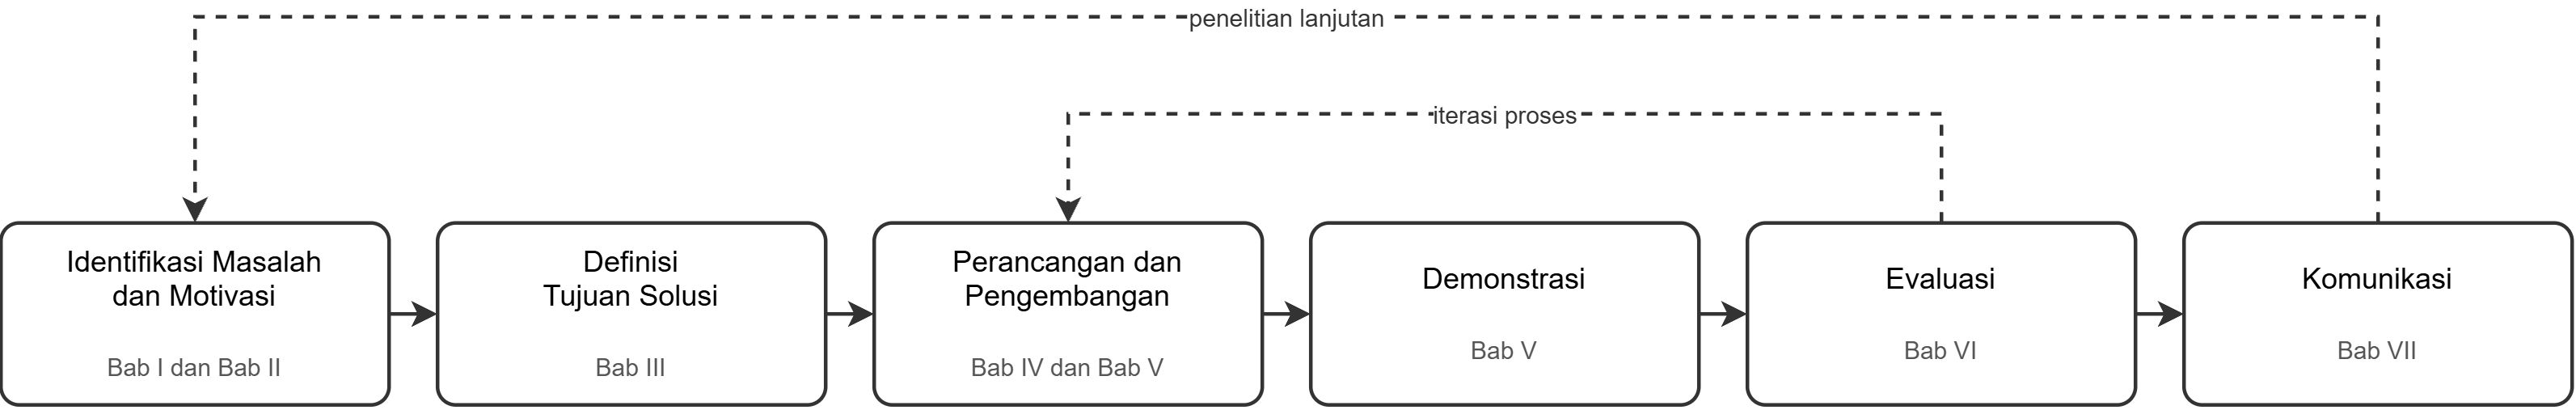
\includegraphics[width=0.8\textwidth]{images/bab1/fig1.1_dsrm.png}
    \caption[Enam aktivitas \textit{Design Science Research Methodology} dan pemetaannya terhadap struktur laporan tugas akhir.]{Enam aktivitas \textit{Design Science Research Methodology} dan pemetaannya terhadap struktur laporan tugas akhir (Diadaptasi dari \citeauthor{peffers2007} \citeyear{peffers2007}).}
    \label{fig:fig1.1_dsrm}
\end{figure}

Dalam pemetaan tersebut, evaluasi adalah aktivitas penelitian yang menguji artefak, bukan salah satu tujuan artefak. Karena itu, tujuan penelitian hanya memuat tiga
artefak (T1 sampai T3), sedangkan evaluasi terhadap ketiganya dilaporkan tersendiri pada Bab VI.

\section{Kontribusi Penelitian}
\label{sec:bab1-kontribusi}
Penelitian ini memberikan tiga kontribusi berupa artefak dan satu kontribusi empiris.

\begin{enumerate}
    \item \textbf{Mekanisme \textit{query transformation} terkondisi-prediksi.} Penelitian menghasilkan mekanisme yang menggunakan kondisi glukosa terprediksi sebagai dasar 
    pengondisian kueri sebelum penelusuran pedoman klinis.

    \item \textbf{Modul prediksi kadar glukosa berbasis data pemantauan.} Penelitian menghasilkan modul prediksi yang dirancang untuk data pemantauan dengan kerapatan
    berbeda dan dapat berjalan pada lingkungan komputasi terbatas.

    \item \textbf{Integrasi CDSS \textit{doctor-mediated}.} Penelitian menghasilkan integrasi prediksi dan retrieval ke dalam alur pendukung keputusan klinis yang 
    menempatkan dokter sebagai pengambil keputusan akhir.

    \item \textbf{Bukti empiris mengenai RAG terkondisi-prediksi.} Penelitian menyediakan evaluasi yang membandingkan mekanisme terkondisi-prediksi dengan RAG standar. Klaim
    mengenai keunggulan atau keterbatasan mekanisme tersebut ditentukan dari hasil evaluasi, bukan diasumsikan sejak awal.
\end{enumerate}

\section{Sistematika Penulisan}
\label{sec:bab1-sistematika}

Laporan tugas akhir ini terdiri atas tujuh bab.

\textbf{Bab I Pendahuluan} menjelaskan konteks masalah, \textit{research gap}, rumusan masalah, tujuan penelitian, batasan masalah, metodologi, kontribusi, dan sistematika 
penulisan.

\textbf{Bab II Studi Literatur} membahas dasar ilmiah mengenai DMT1, pemantauan glukosa, karakteristik dan pemodelan data glukosa, metode prediksi, evaluasi dan ketidakpastian 
prediksi, CDSS, RAG, \textit{grounded generation}, evaluasi RAG, penelitian terkait, \textit{research gap}, dan posisi penelitian.

\textbf{Bab III Analisis Masalah} menguraikan kondisi saat ini, persoalan, kebutuhan pengguna dan sistem, analisis data, alternatif pendekatan, serta keputusan solusi yang 
diturunkan dari kebutuhan.

\textbf{Bab IV Perancangan Sistem RAG Terkondisi-Prediksi} menjelaskan rancangan arsitektur, modul prediksi, mekanisme RAG terkondisi-prediksi, dan integrasi CDSS.

\textbf{Bab V Implementasi Sistem RAG Terkondisi-Prediksi} menjelaskan realisasi rancangan menjadi sistem yang dapat dijalankan, termasuk lingkungan implementasi, implementasi modul prediksi, 
implementasi RAG, integrasi CDSS, demonstrasi, dan verifikasi fungsional.

\textbf{Bab VI Evaluasi Sistem RAG Terkondisi-Prediksi} menyajikan rancangan dan hasil evaluasi terhadap ketiga tujuan artefak, mencakup prediksi, \textit{retrieval} dan \textit{generation}, keamanan
klinis, kinerja operasional, ketahanan sistem, serta evaluasi ahli sesuai ruang lingkup penelitian.

\textbf{Bab VII Penutup} menyajikan kesimpulan berdasarkan ketiga tujuan penelitian, pemenuhan kebutuhan sistem, keterbatasan penelitian, dan saran pengembangan lebih lanjut.